% import macros and common styles
\documentclass[11pt]{article}
\usepackage[margin=1in]{geometry}
\usepackage{fancyhdr}
\usepackage[noindentafter]{titlesec}
\usepackage[T1]{fontenc}
\usepackage[scaled]{helvet}
\usepackage[pdftex]{graphicx}
\usepackage{subfigure}
\usepackage[subfigure]{tocloft}
\usepackage{etoc}
\usepackage{float}
\usepackage{amsmath}
\usepackage{changepage}
\usepackage{subfiles}
\usepackage{tabularx}
\usepackage{threeparttable}
\usepackage{caption}
\usepackage{longtable}
\usepackage{tcolorbox}
\usepackage{listings}
\usepackage{color}
\usepackage{hyperref}



\newcommand{\alertbox}[1]{\begin{tcolorbox}[colback=red!5!white,colframe=red!75!black,title=Alert]#1\end{tcolorbox}}


% code block
\definecolor{darkorange}{rgb}{0.99,0.91,0.85}
\definecolor{gray}{rgb}{0.6,0.6,0.6}

\lstset{
	language=C++,
	basicstyle=\fontfamily{NotoSansMono-TLF}\small,
	frame=single,
	showstringspaces=false,
	numbers=none,
	backgroundcolor=\color{darkorange},
	commentstyle=\color{gray},
	linewidth=1\linewidth,
	aboveskip=12pt,
	belowskip=12pt,
	tabsize=4,
	morekeywords={VESSEL, VESSEL2, VESSEL3, VESSEL4, HINSTANCE, OBJHANDLE, FILEHANDLE, PROPELLANT_HANDLE, THRUSTER_HANDLE, SURFHANDLE, DWORD, UINT, ANIMATIONCOMPONENT_HANDLE, MGROUP_ROTATE, MGROUP_TRANSLATE, MGROUP_SCALE}
}



\graphicspath{{Images//}{../Orbiter Technical Reference/}{../Orbiter Technical Reference/Images//}}
% eps figures come from the Windows edition's folder: convert them into this folder, the path has spaces
\usepackage{epstopdf}
\epstopdfsetup{outdir=./}
\epstopdfDeclareGraphicsRule{.eps}{pdf}{.pdf}{repstopdf "#1" --outfile=\OutputFile}
\bibliographystyle{unsrt}


\renewcommand*\familydefault{\sfdefault}
\sffamily

\pagestyle{fancy}
\renewcommand{\footrulewidth}{0.4pt}


% define page header/footer
\lhead{}
\chead{}
\rhead{}
\lfoot{Orbiter Technical Reference (Linux)}
\cfoot{\thepage}


\titleformat{\paragraph}[hang]{\bfseries}{\theparagraph}{1em}{}



\begin{document}

\begin{titlepage}
\begin{center}


\textsc{\fontsize{60}{60} \textbf{Orbiter}}\\
\vspace{0.5cm}

\textsc{\Huge Space Flight Simulator}\\
\vspace{2.0cm}

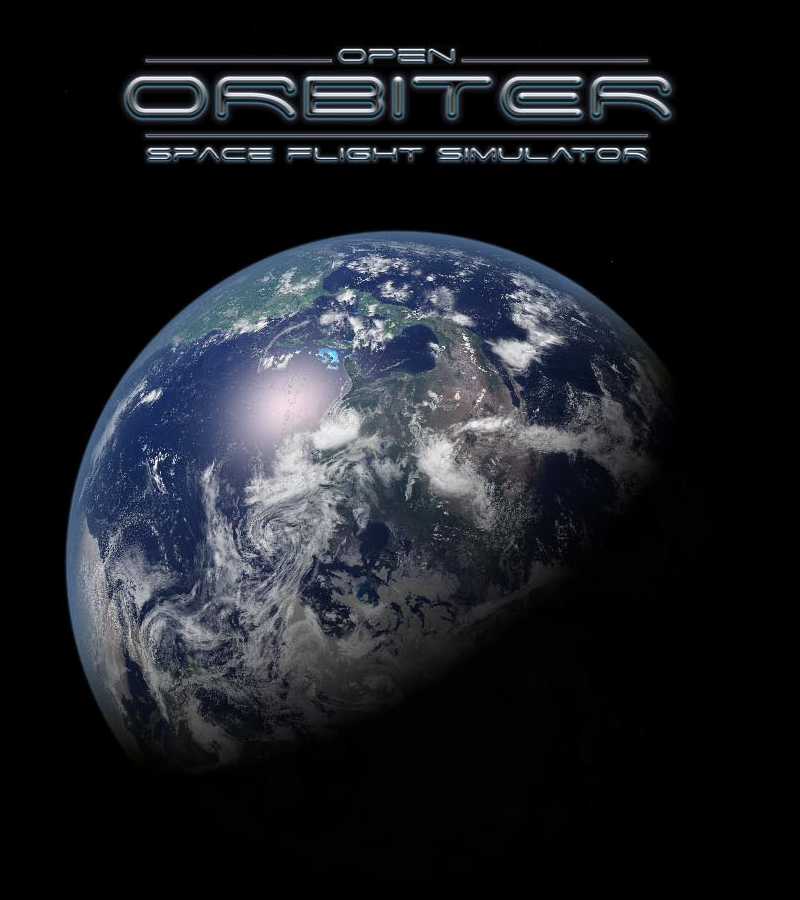
\includegraphics[width=0.75\textwidth]{..//orbiterlogo.png}
\vspace{2.0cm}

\textsc{\LARGE Orbiter Technical Reference}\\
\vspace{0.5cm}
\textsc{\Large Linux edition}

\end{center}
\end{titlepage}


\newpage
\pagenumbering{roman}

\tableofcontents
\newpage

\pagenumbering{arabic}

\newpage
\subfile{INTRODUCTION}
\newpage
\subfile{composite}
\newpage
\subfile{distmass}
\newpage
\subfile{dynamics}
\newpage
\subfile{dynsurf}
\newpage
\subfile{earth_atm}
\newpage
\subfile{gravity}
\newpage
\subfile{lighting}
\newpage
\subfile{precession}
\newpage
\subfile{RecorderRef}
\newpage
\bibliography{REFERENCES}

\end{document}